\documentclass{standalone}
\usepackage{tikz}
\usepackage{pgfplots}
\pgfplotsset{compat=1.12,width=5cm}%
\begin{document}
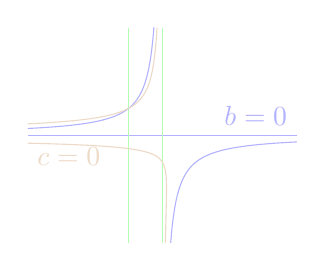
\begin{tikzpicture}
\newcommand{\mx}{4}
\begin{axis}[hide axis,xmin=-\mx,xmax=\mx,ymin=-\mx,ymax=\mx]
\newcommand{\fclr}{blue!30}
\draw[\fclr] 
	(-\mx,0) 
-- (\mx,0) node[above left]{\(b=0\)};
\newcommand{\gclr}{brown!30}
\draw[green!30] (0,-\mx) -- (0,\mx);
\draw[green!30] (-1,-\mx) -- (-1,\mx);
  \addplot[domain=-\mx:-.1,\fclr,samples=200]{-1/x};%
  \addplot[domain=.1:\mx,\fclr,samples=200]{-1/x};%
  \addplot[domain=.1:\mx,\gclr,samples=200]({(-x-1)/(2*x^2)},{x});
  \addplot[domain=-\mx:-.1,\gclr,samples=200]({(-x-1)/(2*x^2)},{x});
  \node[\gclr,below right] at (-\mx,-.1) {\(c=0\)};
\end{axis}
\end{tikzpicture}
\end{document}
